% Created by tikzDevice version 0.11 on 2018-07-24 15:50:23
% !TEX encoding = UTF-8 Unicode
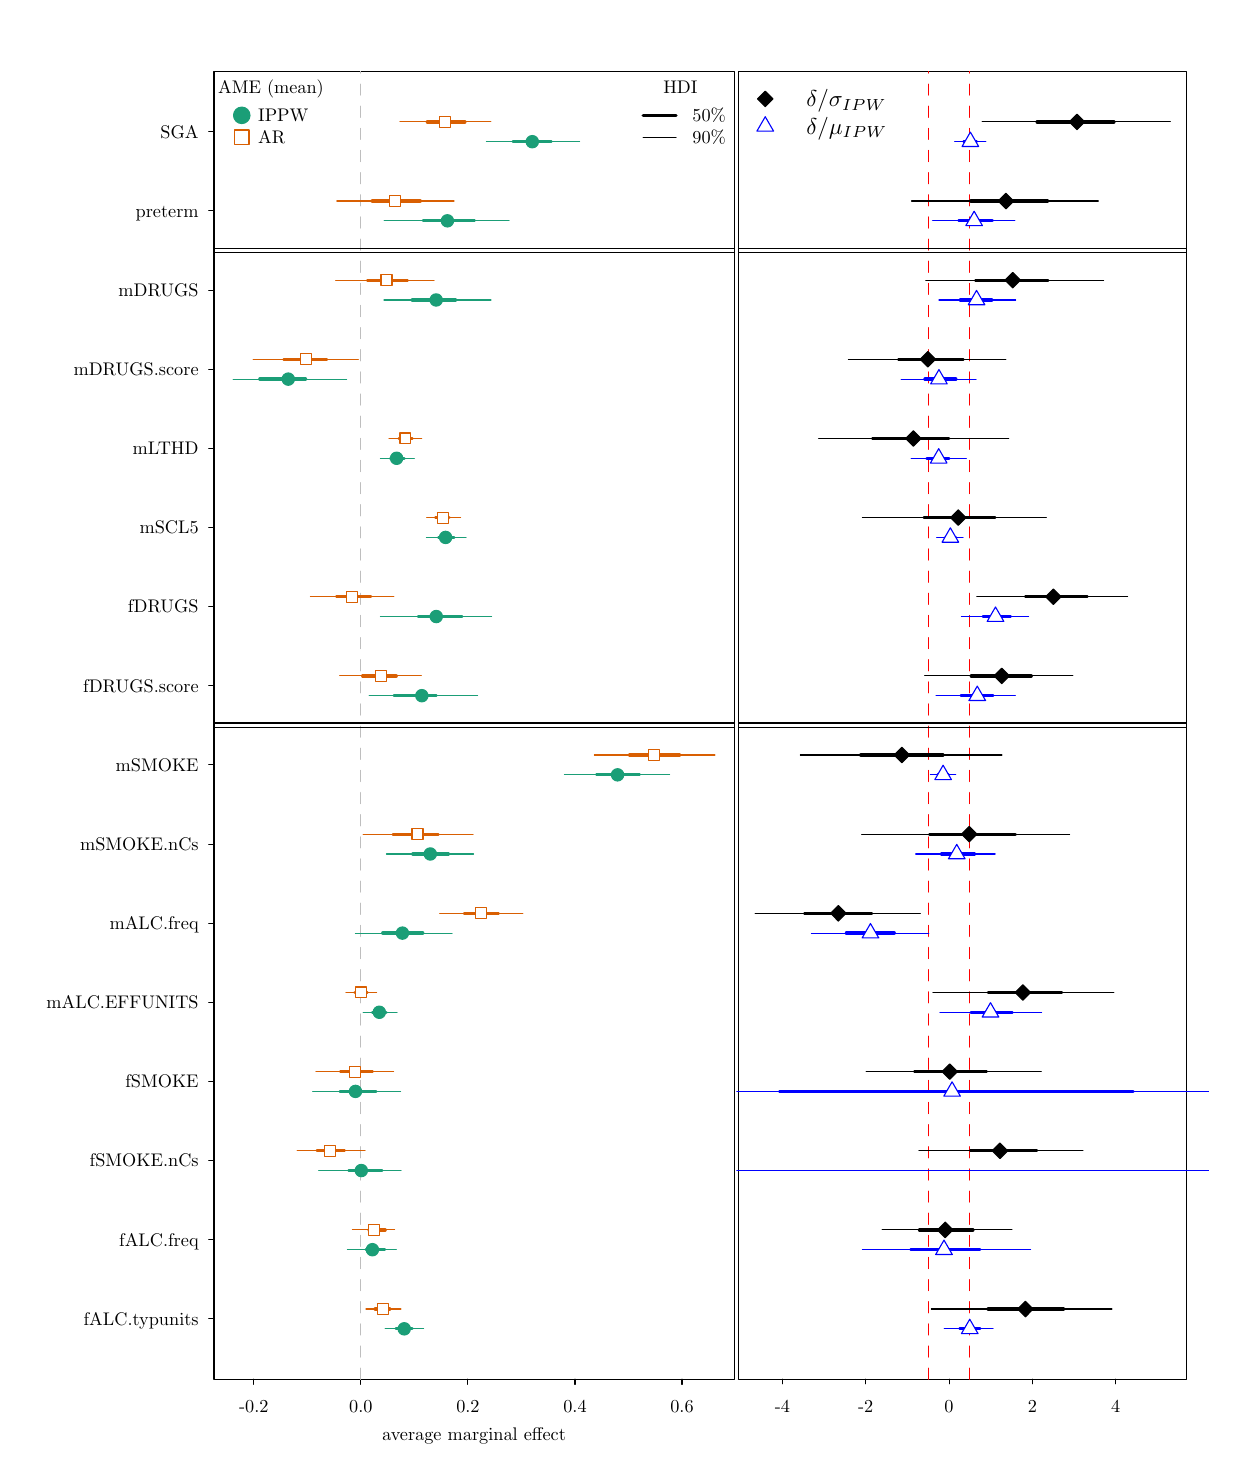
\begin{tikzpicture}[x=1pt,y=1pt]
\definecolor{fillColor}{RGB}{255,255,255}
\path[use as bounding box,fill=fillColor,fill opacity=0.00] (0,0) rectangle (426.79,512.15);
\begin{scope}
\path[clip] (  0.00,  0.00) rectangle (426.79,512.15);
\definecolor{drawColor}{RGB}{0,0,0}

\path[draw=drawColor,line width= 0.4pt,line join=round,line cap=round] ( 81.73, 23.76) -- (236.45, 23.76);

\path[draw=drawColor,line width= 0.4pt,line join=round,line cap=round] ( 81.73, 23.76) -- ( 81.73, 21.88);

\path[draw=drawColor,line width= 0.4pt,line join=round,line cap=round] (120.41, 23.76) -- (120.41, 21.88);

\path[draw=drawColor,line width= 0.4pt,line join=round,line cap=round] (159.09, 23.76) -- (159.09, 21.88);

\path[draw=drawColor,line width= 0.4pt,line join=round,line cap=round] (197.77, 23.76) -- (197.77, 21.88);

\path[draw=drawColor,line width= 0.4pt,line join=round,line cap=round] (236.45, 23.76) -- (236.45, 21.88);

\node[text=drawColor,anchor=base,inner sep=0pt, outer sep=0pt, scale=  0.66] at ( 81.73, 11.88) {-0.2};

\node[text=drawColor,anchor=base,inner sep=0pt, outer sep=0pt, scale=  0.66] at (120.41, 11.88) {0.0};

\node[text=drawColor,anchor=base,inner sep=0pt, outer sep=0pt, scale=  0.66] at (159.09, 11.88) {0.2};

\node[text=drawColor,anchor=base,inner sep=0pt, outer sep=0pt, scale=  0.66] at (197.77, 11.88) {0.4};

\node[text=drawColor,anchor=base,inner sep=0pt, outer sep=0pt, scale=  0.66] at (236.45, 11.88) {0.6};

\path[draw=drawColor,line width= 0.4pt,line join=round,line cap=round] ( 67.32, 23.76) --
	(255.28, 23.76) --
	(255.28,496.31) --
	( 67.32,496.31) --
	( 67.32, 23.76);
\end{scope}
\begin{scope}
\path[clip] (  0.00,  0.00) rectangle (256.07,512.15);
\definecolor{drawColor}{RGB}{0,0,0}

\node[text=drawColor,anchor=base,inner sep=0pt, outer sep=0pt, scale=  0.66] at (161.30,  1.58) {average marginal effect};
\end{scope}
\begin{scope}
\path[clip] ( 67.32, 23.76) rectangle (255.28,496.31);
\definecolor{drawColor}{RGB}{190,190,190}

\path[draw=drawColor,line width= 0.4pt,dash pattern=on 4pt off 4pt ,line join=round,line cap=round] (120.41, 23.76) -- (120.41,496.31);
\definecolor{drawColor}{RGB}{27,158,119}

\path[draw=drawColor,line width= 1.2pt,line join=round,line cap=round] (175.33,470.94) -- (189.22,470.94);

\path[draw=drawColor,line width= 1.2pt,line join=round,line cap=round] (142.87,442.35) -- (161.46,442.35);

\path[draw=drawColor,line width= 1.2pt,line join=round,line cap=round] (138.95,413.75) -- (154.58,413.75);

\path[draw=drawColor,line width= 1.2pt,line join=round,line cap=round] ( 83.89,385.15) -- (100.40,385.15);

\path[draw=drawColor,line width= 1.2pt,line join=round,line cap=round] (131.05,356.55) -- (136.06,356.55);

\path[draw=drawColor,line width= 1.2pt,line join=round,line cap=round] (148.43,327.95) -- (154.09,327.95);

\path[draw=drawColor,line width= 1.2pt,line join=round,line cap=round] (141.09,299.36) -- (156.98,299.36);

\path[draw=drawColor,line width= 1.2pt,line join=round,line cap=round] (132.35,270.76) -- (147.68,270.76);

\path[draw=drawColor,line width= 1.2pt,line join=round,line cap=round] (205.51,242.16) -- (221.12,242.16);

\path[draw=drawColor,line width= 1.2pt,line join=round,line cap=round] (139.19,213.56) -- (152.00,213.56);

\path[draw=drawColor,line width= 1.2pt,line join=round,line cap=round] (128.30,184.97) -- (142.75,184.97);

\path[draw=drawColor,line width= 1.2pt,line join=round,line cap=round] (124.54,156.37) -- (129.55,156.37);

\path[draw=drawColor,line width= 1.2pt,line join=round,line cap=round] (112.85,127.77) -- (125.88,127.77);

\path[draw=drawColor,line width= 1.2pt,line join=round,line cap=round] (116.00, 99.17) -- (128.07, 99.17);

\path[draw=drawColor,line width= 1.2pt,line join=round,line cap=round] (122.24, 70.57) -- (129.02, 70.57);

\path[draw=drawColor,line width= 1.2pt,line join=round,line cap=round] (133.09, 41.98) -- (138.95, 41.98);

\path[draw=drawColor,line width= 0.4pt,line join=round,line cap=round] (165.78,470.94) -- (199.46,470.94);

\path[draw=drawColor,line width= 0.4pt,line join=round,line cap=round] (128.81,442.35) -- (173.96,442.35);

\path[draw=drawColor,line width= 0.4pt,line join=round,line cap=round] (128.76,413.75) -- (167.41,413.75);

\path[draw=drawColor,line width= 0.4pt,line join=round,line cap=round] ( 74.28,385.15) -- (115.23,385.15);

\path[draw=drawColor,line width= 0.4pt,line join=round,line cap=round] (127.47,356.55) -- (139.76,356.55);

\path[draw=drawColor,line width= 0.4pt,line join=round,line cap=round] (144.12,327.95) -- (158.43,327.95);

\path[draw=drawColor,line width= 0.4pt,line join=round,line cap=round] (127.46,299.36) -- (167.62,299.36);

\path[draw=drawColor,line width= 0.4pt,line join=round,line cap=round] (123.42,270.76) -- (162.54,270.76);

\path[draw=drawColor,line width= 0.4pt,line join=round,line cap=round] (193.96,242.16) -- (231.99,242.16);

\path[draw=drawColor,line width= 0.4pt,line join=round,line cap=round] (129.64,213.56) -- (161.10,213.56);

\path[draw=drawColor,line width= 0.4pt,line join=round,line cap=round] (118.46,184.97) -- (153.33,184.97);

\path[draw=drawColor,line width= 0.4pt,line join=round,line cap=round] (121.20,156.37) -- (133.47,156.37);

\path[draw=drawColor,line width= 0.4pt,line join=round,line cap=round] (102.98,127.77) -- (134.74,127.77);

\path[draw=drawColor,line width= 0.4pt,line join=round,line cap=round] (105.17, 99.17) -- (134.93, 99.17);

\path[draw=drawColor,line width= 0.4pt,line join=round,line cap=round] (115.51, 70.57) -- (133.20, 70.57);

\path[draw=drawColor,line width= 0.4pt,line join=round,line cap=round] (129.17, 41.98) -- (143.08, 41.98);
\definecolor{fillColor}{RGB}{27,158,119}

\path[draw=drawColor,line width= 0.4pt,line join=round,line cap=round,fill=fillColor] (182.34,470.94) circle (  2.23);

\path[draw=drawColor,line width= 0.4pt,line join=round,line cap=round,fill=fillColor] (151.67,442.35) circle (  2.23);

\path[draw=drawColor,line width= 0.4pt,line join=round,line cap=round,fill=fillColor] (147.61,413.75) circle (  2.23);

\path[draw=drawColor,line width= 0.4pt,line join=round,line cap=round,fill=fillColor] ( 94.16,385.15) circle (  2.23);

\path[draw=drawColor,line width= 0.4pt,line join=round,line cap=round,fill=fillColor] (133.31,356.55) circle (  2.23);

\path[draw=drawColor,line width= 0.4pt,line join=round,line cap=round,fill=fillColor] (151.01,327.95) circle (  2.23);

\path[draw=drawColor,line width= 0.4pt,line join=round,line cap=round,fill=fillColor] (147.64,299.36) circle (  2.23);

\path[draw=drawColor,line width= 0.4pt,line join=round,line cap=round,fill=fillColor] (142.43,270.76) circle (  2.23);

\path[draw=drawColor,line width= 0.4pt,line join=round,line cap=round,fill=fillColor] (213.15,242.16) circle (  2.23);

\path[draw=drawColor,line width= 0.4pt,line join=round,line cap=round,fill=fillColor] (145.48,213.56) circle (  2.23);

\path[draw=drawColor,line width= 0.4pt,line join=round,line cap=round,fill=fillColor] (135.42,184.97) circle (  2.23);

\path[draw=drawColor,line width= 0.4pt,line join=round,line cap=round,fill=fillColor] (127.07,156.37) circle (  2.23);

\path[draw=drawColor,line width= 0.4pt,line join=round,line cap=round,fill=fillColor] (118.44,127.77) circle (  2.23);

\path[draw=drawColor,line width= 0.4pt,line join=round,line cap=round,fill=fillColor] (120.56, 99.17) circle (  2.23);

\path[draw=drawColor,line width= 0.4pt,line join=round,line cap=round,fill=fillColor] (124.57, 70.57) circle (  2.23);

\path[draw=drawColor,line width= 0.4pt,line join=round,line cap=round,fill=fillColor] (136.07, 41.98) circle (  2.23);
\definecolor{drawColor}{RGB}{217,95,2}

\path[draw=drawColor,line width= 1.2pt,line join=round,line cap=round] (144.42,478.09) -- (157.97,478.09);

\path[draw=drawColor,line width= 1.2pt,line join=round,line cap=round] (124.49,449.50) -- (141.84,449.50);

\path[draw=drawColor,line width= 1.2pt,line join=round,line cap=round] (122.73,420.90) -- (137.26,420.90);

\path[draw=drawColor,line width= 1.2pt,line join=round,line cap=round] ( 92.52,392.30) -- (108.08,392.30);

\path[draw=drawColor,line width= 1.2pt,line join=round,line cap=round] (134.16,363.70) -- (138.97,363.70);

\path[draw=drawColor,line width= 1.2pt,line join=round,line cap=round] (147.35,335.10) -- (152.31,335.10);

\path[draw=drawColor,line width= 1.2pt,line join=round,line cap=round] (111.54,306.51) -- (124.03,306.51);

\path[draw=drawColor,line width= 1.2pt,line join=round,line cap=round] (121.04,277.91) -- (133.17,277.91);

\path[draw=drawColor,line width= 1.2pt,line join=round,line cap=round] (217.51,249.31) -- (235.54,249.31);

\path[draw=drawColor,line width= 1.2pt,line join=round,line cap=round] (131.96,220.71) -- (148.38,220.71);

\path[draw=drawColor,line width= 1.2pt,line join=round,line cap=round] (157.74,192.12) -- (170.18,192.12);

\path[draw=drawColor,line width= 1.2pt,line join=round,line cap=round] (118.21,163.52) -- (122.75,163.52);

\path[draw=drawColor,line width= 1.2pt,line join=round,line cap=round] (112.98,134.92) -- (124.62,134.92);

\path[draw=drawColor,line width= 1.2pt,line join=round,line cap=round] (104.50,106.32) -- (114.48,106.32);

\path[draw=drawColor,line width= 1.2pt,line join=round,line cap=round] (123.36, 77.72) -- (129.17, 77.72);

\path[draw=drawColor,line width= 1.2pt,line join=round,line cap=round] (125.57, 49.13) -- (130.80, 49.13);

\path[draw=drawColor,line width= 0.4pt,line join=round,line cap=round] (134.51,478.09) -- (167.37,478.09);

\path[draw=drawColor,line width= 0.4pt,line join=round,line cap=round] (111.72,449.50) -- (154.06,449.50);

\path[draw=drawColor,line width= 0.4pt,line join=round,line cap=round] (111.26,420.90) -- (146.87,420.90);

\path[draw=drawColor,line width= 0.4pt,line join=round,line cap=round] ( 81.47,392.30) -- (119.49,392.30);

\path[draw=drawColor,line width= 0.4pt,line join=round,line cap=round] (130.57,363.70) -- (142.38,363.70);

\path[draw=drawColor,line width= 0.4pt,line join=round,line cap=round] (144.16,335.10) -- (156.44,335.10);

\path[draw=drawColor,line width= 0.4pt,line join=round,line cap=round] (102.16,306.51) -- (132.30,306.51);

\path[draw=drawColor,line width= 0.4pt,line join=round,line cap=round] (112.72,277.91) -- (142.22,277.91);

\path[draw=drawColor,line width= 0.4pt,line join=round,line cap=round] (204.77,249.31) -- (248.32,249.31);

\path[draw=drawColor,line width= 0.4pt,line join=round,line cap=round] (121.26,220.71) -- (160.95,220.71);

\path[draw=drawColor,line width= 0.4pt,line join=round,line cap=round] (148.87,192.12) -- (178.91,192.12);

\path[draw=drawColor,line width= 0.4pt,line join=round,line cap=round] (114.98,163.52) -- (126.07,163.52);

\path[draw=drawColor,line width= 0.4pt,line join=round,line cap=round] (104.12,134.92) -- (132.21,134.92);

\path[draw=drawColor,line width= 0.4pt,line join=round,line cap=round] ( 97.41,106.32) -- (121.89,106.32);

\path[draw=drawColor,line width= 0.4pt,line join=round,line cap=round] (117.36, 77.72) -- (132.56, 77.72);

\path[draw=drawColor,line width= 0.4pt,line join=round,line cap=round] (122.25, 49.13) -- (134.87, 49.13);
\definecolor{fillColor}{RGB}{255,255,255}

\path[draw=drawColor,line width= 0.4pt,line join=round,line cap=round,fill=fillColor] (148.70,476.12) rectangle (152.65,480.07);

\path[draw=drawColor,line width= 0.4pt,line join=round,line cap=round,fill=fillColor] (130.88,447.52) rectangle (134.83,451.47);

\path[draw=drawColor,line width= 0.4pt,line join=round,line cap=round,fill=fillColor] (127.69,418.92) rectangle (131.64,422.87);

\path[draw=drawColor,line width= 0.4pt,line join=round,line cap=round,fill=fillColor] ( 98.54,390.33) rectangle (102.49,394.27);

\path[draw=drawColor,line width= 0.4pt,line join=round,line cap=round,fill=fillColor] (134.54,361.73) rectangle (138.49,365.68);

\path[draw=drawColor,line width= 0.4pt,line join=round,line cap=round,fill=fillColor] (148.07,333.13) rectangle (152.02,337.08);

\path[draw=drawColor,line width= 0.4pt,line join=round,line cap=round,fill=fillColor] (115.31,304.53) rectangle (119.26,308.48);

\path[draw=drawColor,line width= 0.4pt,line join=round,line cap=round,fill=fillColor] (125.55,275.93) rectangle (129.50,279.88);

\path[draw=drawColor,line width= 0.4pt,line join=round,line cap=round,fill=fillColor] (224.38,247.34) rectangle (228.33,251.28);

\path[draw=drawColor,line width= 0.4pt,line join=round,line cap=round,fill=fillColor] (138.88,218.74) rectangle (142.83,222.69);

\path[draw=drawColor,line width= 0.4pt,line join=round,line cap=round,fill=fillColor] (161.75,190.14) rectangle (165.70,194.09);

\path[draw=drawColor,line width= 0.4pt,line join=round,line cap=round,fill=fillColor] (118.47,161.54) rectangle (122.42,165.49);

\path[draw=drawColor,line width= 0.4pt,line join=round,line cap=round,fill=fillColor] (116.32,132.95) rectangle (120.27,136.89);

\path[draw=drawColor,line width= 0.4pt,line join=round,line cap=round,fill=fillColor] (107.23,104.35) rectangle (111.18,108.30);

\path[draw=drawColor,line width= 0.4pt,line join=round,line cap=round,fill=fillColor] (123.10, 75.75) rectangle (127.05, 79.70);

\path[draw=drawColor,line width= 0.4pt,line join=round,line cap=round,fill=fillColor] (126.32, 47.15) rectangle (130.27, 51.10);
\end{scope}
\begin{scope}
\path[clip] (  0.00,  0.00) rectangle (426.79,512.15);
\definecolor{drawColor}{RGB}{0,0,0}

\path[draw=drawColor,line width= 0.4pt,line join=round,line cap=round] ( 67.32, 45.55) -- ( 67.32,474.52);

\path[draw=drawColor,line width= 0.4pt,line join=round,line cap=round] ( 67.32, 45.55) -- ( 65.44, 45.55);

\path[draw=drawColor,line width= 0.4pt,line join=round,line cap=round] ( 67.32, 74.15) -- ( 65.44, 74.15);

\path[draw=drawColor,line width= 0.4pt,line join=round,line cap=round] ( 67.32,102.75) -- ( 65.44,102.75);

\path[draw=drawColor,line width= 0.4pt,line join=round,line cap=round] ( 67.32,131.34) -- ( 65.44,131.34);

\path[draw=drawColor,line width= 0.4pt,line join=round,line cap=round] ( 67.32,159.94) -- ( 65.44,159.94);

\path[draw=drawColor,line width= 0.4pt,line join=round,line cap=round] ( 67.32,188.54) -- ( 65.44,188.54);

\path[draw=drawColor,line width= 0.4pt,line join=round,line cap=round] ( 67.32,217.14) -- ( 65.44,217.14);

\path[draw=drawColor,line width= 0.4pt,line join=round,line cap=round] ( 67.32,245.74) -- ( 65.44,245.74);

\path[draw=drawColor,line width= 0.4pt,line join=round,line cap=round] ( 67.32,274.33) -- ( 65.44,274.33);

\path[draw=drawColor,line width= 0.4pt,line join=round,line cap=round] ( 67.32,302.93) -- ( 65.44,302.93);

\path[draw=drawColor,line width= 0.4pt,line join=round,line cap=round] ( 67.32,331.53) -- ( 65.44,331.53);

\path[draw=drawColor,line width= 0.4pt,line join=round,line cap=round] ( 67.32,360.13) -- ( 65.44,360.13);

\path[draw=drawColor,line width= 0.4pt,line join=round,line cap=round] ( 67.32,388.72) -- ( 65.44,388.72);

\path[draw=drawColor,line width= 0.4pt,line join=round,line cap=round] ( 67.32,417.32) -- ( 65.44,417.32);

\path[draw=drawColor,line width= 0.4pt,line join=round,line cap=round] ( 67.32,445.92) -- ( 65.44,445.92);

\path[draw=drawColor,line width= 0.4pt,line join=round,line cap=round] ( 67.32,474.52) -- ( 65.44,474.52);

\node[text=drawColor,anchor=base east,inner sep=0pt, outer sep=0pt, scale=  0.66] at ( 61.78, 43.28) {fALC.typunits};

\node[text=drawColor,anchor=base east,inner sep=0pt, outer sep=0pt, scale=  0.66] at ( 61.78, 71.88) {fALC.freq};

\node[text=drawColor,anchor=base east,inner sep=0pt, outer sep=0pt, scale=  0.66] at ( 61.78,100.47) {fSMOKE.nCs};

\node[text=drawColor,anchor=base east,inner sep=0pt, outer sep=0pt, scale=  0.66] at ( 61.78,129.07) {fSMOKE};

\node[text=drawColor,anchor=base east,inner sep=0pt, outer sep=0pt, scale=  0.66] at ( 61.78,157.67) {mALC.EFFUNITS};

\node[text=drawColor,anchor=base east,inner sep=0pt, outer sep=0pt, scale=  0.66] at ( 61.78,186.27) {mALC.freq};

\node[text=drawColor,anchor=base east,inner sep=0pt, outer sep=0pt, scale=  0.66] at ( 61.78,214.87) {mSMOKE.nCs};

\node[text=drawColor,anchor=base east,inner sep=0pt, outer sep=0pt, scale=  0.66] at ( 61.78,243.46) {mSMOKE};

\node[text=drawColor,anchor=base east,inner sep=0pt, outer sep=0pt, scale=  0.66] at ( 61.78,272.06) {fDRUGS.score};

\node[text=drawColor,anchor=base east,inner sep=0pt, outer sep=0pt, scale=  0.66] at ( 61.78,300.66) {fDRUGS};

\node[text=drawColor,anchor=base east,inner sep=0pt, outer sep=0pt, scale=  0.66] at ( 61.78,329.26) {mSCL5};

\node[text=drawColor,anchor=base east,inner sep=0pt, outer sep=0pt, scale=  0.66] at ( 61.78,357.85) {mLTHD};

\node[text=drawColor,anchor=base east,inner sep=0pt, outer sep=0pt, scale=  0.66] at ( 61.78,386.45) {mDRUGS.score};

\node[text=drawColor,anchor=base east,inner sep=0pt, outer sep=0pt, scale=  0.66] at ( 61.78,415.05) {mDRUGS};

\node[text=drawColor,anchor=base east,inner sep=0pt, outer sep=0pt, scale=  0.66] at ( 61.78,443.65) {preterm};

\node[text=drawColor,anchor=base east,inner sep=0pt, outer sep=0pt, scale=  0.66] at ( 61.78,472.25) {SGA};
\end{scope}
\begin{scope}
\path[clip] ( 67.32, 23.76) rectangle (255.28,496.31);
\definecolor{drawColor}{RGB}{27,158,119}
\definecolor{fillColor}{RGB}{27,158,119}

\path[draw=drawColor,line width= 0.4pt,line join=round,line cap=round,fill=fillColor] ( 77.36,480.47) circle (  2.97);
\definecolor{drawColor}{RGB}{217,95,2}
\definecolor{fillColor}{RGB}{255,255,255}

\path[draw=drawColor,line width= 0.4pt,line join=round,line cap=round,fill=fillColor] ( 74.72,469.92) rectangle ( 79.99,475.18);
\definecolor{drawColor}{RGB}{0,0,0}

\node[text=drawColor,anchor=base,inner sep=0pt, outer sep=0pt, scale=  0.66] at ( 87.91,488.39) {AME (mean)};

\node[text=drawColor,anchor=base west,inner sep=0pt, outer sep=0pt, scale=  0.66] at ( 83.30,478.20) {IPPW};

\node[text=drawColor,anchor=base west,inner sep=0pt, outer sep=0pt, scale=  0.66] at ( 83.30,470.28) {AR};

\path[draw=drawColor,line width= 1.2pt,line join=round,line cap=round] (222.40,480.47) -- (234.28,480.47);

\path[draw=drawColor,line width= 0.4pt,line join=round,line cap=round] (222.40,472.55) -- (234.28,472.55);

\node[text=drawColor,anchor=base,inner sep=0pt, outer sep=0pt, scale=  0.66] at (235.87,488.39) {HDI};

\node[text=drawColor,anchor=base west,inner sep=0pt, outer sep=0pt, scale=  0.66] at (240.22,478.20) {50\%};

\node[text=drawColor,anchor=base west,inner sep=0pt, outer sep=0pt, scale=  0.66] at (240.22,470.28) {90\%};

\path[draw=drawColor,line width= 0.4pt,line join=round,line cap=round] ( 67.32,430.76) -- (255.28,430.76);

\path[draw=drawColor,line width= 0.4pt,line join=round,line cap=round] ( 67.32,432.48) -- (255.28,432.48);

\path[draw=drawColor,line width= 0.4pt,line join=round,line cap=round] ( 67.32,259.18) -- (255.28,259.18);

\path[draw=drawColor,line width= 0.4pt,line join=round,line cap=round] ( 67.32,260.89) -- (255.28,260.89);
\end{scope}
\begin{scope}
\path[clip] (  0.00,  0.00) rectangle (426.79,512.15);
\definecolor{drawColor}{RGB}{0,0,0}

\path[draw=drawColor,line width= 0.4pt,line join=round,line cap=round] (272.72, 23.76) -- (393.15, 23.76);

\path[draw=drawColor,line width= 0.4pt,line join=round,line cap=round] (272.72, 23.76) -- (272.72, 22.14);

\path[draw=drawColor,line width= 0.4pt,line join=round,line cap=round] (302.83, 23.76) -- (302.83, 22.14);

\path[draw=drawColor,line width= 0.4pt,line join=round,line cap=round] (332.94, 23.76) -- (332.94, 22.14);

\path[draw=drawColor,line width= 0.4pt,line join=round,line cap=round] (363.05, 23.76) -- (363.05, 22.14);

\path[draw=drawColor,line width= 0.4pt,line join=round,line cap=round] (393.15, 23.76) -- (393.15, 22.14);

\node[text=drawColor,anchor=base,inner sep=0pt, outer sep=0pt, scale=  0.66] at (272.72, 11.88) {-4};

\node[text=drawColor,anchor=base,inner sep=0pt, outer sep=0pt, scale=  0.66] at (302.83, 11.88) {-2};

\node[text=drawColor,anchor=base,inner sep=0pt, outer sep=0pt, scale=  0.66] at (332.94, 11.88) {0};

\node[text=drawColor,anchor=base,inner sep=0pt, outer sep=0pt, scale=  0.66] at (363.05, 11.88) {2};

\node[text=drawColor,anchor=base,inner sep=0pt, outer sep=0pt, scale=  0.66] at (393.15, 11.88) {4};

\path[draw=drawColor,line width= 0.4pt,line join=round,line cap=round] (256.87, 23.76) --
	(418.87, 23.76) --
	(418.87,496.31) --
	(256.87,496.31) --
	(256.87, 23.76);
\end{scope}
\begin{scope}
\path[clip] (256.87, 23.76) rectangle (418.87,496.31);
\definecolor{drawColor}{RGB}{255,0,0}

\path[draw=drawColor,line width= 0.4pt,dash pattern=on 4pt off 4pt ,line join=round,line cap=round] (325.41, 23.76) -- (325.41,496.31);

\path[draw=drawColor,line width= 0.4pt,dash pattern=on 4pt off 4pt ,line join=round,line cap=round] (340.47, 23.76) -- (340.47,496.31);
\end{scope}
\begin{scope}
\path[clip] (256.07,  0.00) rectangle (426.79,512.15);
\definecolor{drawColor}{RGB}{0,0,0}

\path[draw=drawColor,line width= 0.4pt,line join=round,line cap=round] (344.92,478.09) -- (412.87,478.09);

\path[draw=drawColor,line width= 0.4pt,line join=round,line cap=round] (319.39,449.50) -- (386.85,449.50);

\path[draw=drawColor,line width= 0.4pt,line join=round,line cap=round] (324.53,420.90) -- (388.76,420.90);

\path[draw=drawColor,line width= 0.4pt,line join=round,line cap=round] (296.54,392.30) -- (353.45,392.30);

\path[draw=drawColor,line width= 0.4pt,line join=round,line cap=round] (285.78,363.70) -- (354.49,363.70);

\path[draw=drawColor,line width= 0.4pt,line join=round,line cap=round] (301.63,335.10) -- (368.09,335.10);

\path[draw=drawColor,line width= 0.4pt,line join=round,line cap=round] (342.96,306.51) -- (397.47,306.51);

\path[draw=drawColor,line width= 0.4pt,line join=round,line cap=round] (324.16,277.91) -- (377.63,277.91);

\path[draw=drawColor,line width= 0.4pt,line join=round,line cap=round] (279.20,249.31) -- (352.04,249.31);

\path[draw=drawColor,line width= 0.4pt,line join=round,line cap=round] (301.38,220.71) -- (376.52,220.71);

\path[draw=drawColor,line width= 0.4pt,line join=round,line cap=round] (262.87,192.12) -- (322.58,192.12);

\path[draw=drawColor,line width= 0.4pt,line join=round,line cap=round] (327.08,163.52) -- (392.47,163.52);

\path[draw=drawColor,line width= 0.4pt,line join=round,line cap=round] (303.00,134.92) -- (366.24,134.92);

\path[draw=drawColor,line width= 0.4pt,line join=round,line cap=round] (322.05,106.32) -- (381.32,106.32);

\path[draw=drawColor,line width= 0.4pt,line join=round,line cap=round] (308.74, 77.72) -- (355.67, 77.72);

\path[draw=drawColor,line width= 0.4pt,line join=round,line cap=round] (326.55, 49.13) -- (391.78, 49.13);

\path[draw=drawColor,line width= 1.2pt,line join=round,line cap=round] (364.77,478.09) -- (392.50,478.09);

\path[draw=drawColor,line width= 1.2pt,line join=round,line cap=round] (340.80,449.50) -- (368.51,449.50);

\path[draw=drawColor,line width= 1.2pt,line join=round,line cap=round] (342.45,420.90) -- (368.72,420.90);

\path[draw=drawColor,line width= 1.2pt,line join=round,line cap=round] (314.62,392.30) -- (338.08,392.30);

\path[draw=drawColor,line width= 1.2pt,line join=round,line cap=round] (305.25,363.70) -- (332.89,363.70);

\path[draw=drawColor,line width= 1.2pt,line join=round,line cap=round] (323.86,335.10) -- (349.56,335.10);

\path[draw=drawColor,line width= 1.2pt,line join=round,line cap=round] (360.50,306.51) -- (382.92,306.51);

\path[draw=drawColor,line width= 1.2pt,line join=round,line cap=round] (340.98,277.91) -- (362.62,277.91);

\path[draw=drawColor,line width= 1.2pt,line join=round,line cap=round] (301.02,249.31) -- (330.72,249.31);

\path[draw=drawColor,line width= 1.2pt,line join=round,line cap=round] (325.88,220.71) -- (356.93,220.71);

\path[draw=drawColor,line width= 1.2pt,line join=round,line cap=round] (280.68,192.12) -- (305.02,192.12);

\path[draw=drawColor,line width= 1.2pt,line join=round,line cap=round] (347.04,163.52) -- (373.65,163.52);

\path[draw=drawColor,line width= 1.2pt,line join=round,line cap=round] (320.45,134.92) -- (346.49,134.92);

\path[draw=drawColor,line width= 1.2pt,line join=round,line cap=round] (340.67,106.32) -- (364.64,106.32);

\path[draw=drawColor,line width= 1.2pt,line join=round,line cap=round] (322.25, 77.72) -- (341.55, 77.72);

\path[draw=drawColor,line width= 1.2pt,line join=round,line cap=round] (347.07, 49.13) -- (374.29, 49.13);
\definecolor{drawColor}{RGB}{0,0,255}

\path[draw=drawColor,line width= 0.4pt,line join=round,line cap=round] (334.93,470.94) -- (346.26,470.94);

\path[draw=drawColor,line width= 0.4pt,line join=round,line cap=round] (326.97,442.35) -- (356.70,442.35);

\path[draw=drawColor,line width= 0.4pt,line join=round,line cap=round] (329.31,413.75) -- (357.01,413.75);

\path[draw=drawColor,line width= 0.4pt,line join=round,line cap=round] (315.63,385.15) -- (342.69,385.15);

\path[draw=drawColor,line width= 0.4pt,line join=round,line cap=round] (319.23,356.55) -- (339.20,356.55);

\path[draw=drawColor,line width= 0.4pt,line join=round,line cap=round] (328.42,327.95) -- (338.01,327.95);

\path[draw=drawColor,line width= 0.4pt,line join=round,line cap=round] (337.40,299.36) -- (361.67,299.36);

\path[draw=drawColor,line width= 0.4pt,line join=round,line cap=round] (328.23,270.76) -- (356.87,270.76);

\path[draw=drawColor,line width= 0.4pt,line join=round,line cap=round] (326.19,242.16) -- (335.34,242.16);

\path[draw=drawColor,line width= 0.4pt,line join=round,line cap=round] (320.89,213.56) -- (349.58,213.56);

\path[draw=drawColor,line width= 0.4pt,line join=round,line cap=round] (283.21,184.97) -- (325.59,184.97);

\path[draw=drawColor,line width= 0.4pt,line join=round,line cap=round] (329.65,156.37) -- (366.36,156.37);

\path[draw=drawColor,line width= 0.4pt,line join=round,line cap=round] (185.92,127.77) -- (426.79,127.77);

\path[draw=drawColor,line width= 0.4pt,line join=round,line cap=round] (  0.00, 99.17) -- (426.79, 99.17);

\path[draw=drawColor,line width= 0.4pt,line join=round,line cap=round] (301.59, 70.57) -- (362.39, 70.57);

\path[draw=drawColor,line width= 0.4pt,line join=round,line cap=round] (331.21, 41.98) -- (348.87, 41.98);

\path[draw=drawColor,line width= 1.2pt,line join=round,line cap=round] (338.24,470.94) -- (342.86,470.94);

\path[draw=drawColor,line width= 1.2pt,line join=round,line cap=round] (336.40,442.35) -- (348.62,442.35);

\path[draw=drawColor,line width= 1.2pt,line join=round,line cap=round] (337.04,413.75) -- (348.37,413.75);

\path[draw=drawColor,line width= 1.2pt,line join=round,line cap=round] (324.23,385.15) -- (335.38,385.15);

\path[draw=drawColor,line width= 1.2pt,line join=round,line cap=round] (324.89,356.55) -- (332.92,356.55);

\path[draw=drawColor,line width= 1.2pt,line join=round,line cap=round] (331.63,327.95) -- (335.34,327.95);

\path[draw=drawColor,line width= 1.2pt,line join=round,line cap=round] (345.21,299.36) -- (355.19,299.36);

\path[draw=drawColor,line width= 1.2pt,line join=round,line cap=round] (337.25,270.76) -- (348.83,270.76);

\path[draw=drawColor,line width= 1.2pt,line join=round,line cap=round] (328.93,242.16) -- (332.66,242.16);

\path[draw=drawColor,line width= 1.2pt,line join=round,line cap=round] (330.24,213.56) -- (342.10,213.56);

\path[draw=drawColor,line width= 1.2pt,line join=round,line cap=round] (295.85,184.97) -- (313.13,184.97);

\path[draw=drawColor,line width= 1.2pt,line join=round,line cap=round] (340.85,156.37) -- (355.79,156.37);

\path[draw=drawColor,line width= 1.2pt,line join=round,line cap=round] (271.62,127.77) -- (399.48,127.77);

\path[draw=drawColor,line width= 1.2pt,line join=round,line cap=round] (319.10, 70.57) -- (344.10, 70.57);

\path[draw=drawColor,line width= 1.2pt,line join=round,line cap=round] (336.77, 41.98) -- (344.13, 41.98);
\definecolor{drawColor}{RGB}{0,0,0}
\definecolor{fillColor}{RGB}{0,0,0}

\path[draw=drawColor,line width= 0.4pt,line join=round,line cap=round,fill=fillColor] (379.14,475.30) --
	(381.93,478.09) --
	(379.14,480.88) --
	(376.35,478.09) --
	cycle;

\path[draw=drawColor,line width= 0.4pt,line join=round,line cap=round,fill=fillColor] (353.50,446.70) --
	(356.29,449.50) --
	(353.50,452.29) --
	(350.71,449.50) --
	cycle;

\path[draw=drawColor,line width= 0.4pt,line join=round,line cap=round,fill=fillColor] (355.97,418.11) --
	(358.76,420.90) --
	(355.97,423.69) --
	(353.18,420.90) --
	cycle;

\path[draw=drawColor,line width= 0.4pt,line join=round,line cap=round,fill=fillColor] (325.28,389.51) --
	(328.07,392.30) --
	(325.28,395.09) --
	(322.48,392.30) --
	cycle;

\path[draw=drawColor,line width= 0.4pt,line join=round,line cap=round,fill=fillColor] (320.08,360.91) --
	(322.87,363.70) --
	(320.08,366.49) --
	(317.29,363.70) --
	cycle;

\path[draw=drawColor,line width= 0.4pt,line join=round,line cap=round,fill=fillColor] (336.23,332.31) --
	(339.02,335.10) --
	(336.23,337.90) --
	(333.44,335.10) --
	cycle;

\path[draw=drawColor,line width= 0.4pt,line join=round,line cap=round,fill=fillColor] (370.63,303.71) --
	(373.43,306.51) --
	(370.63,309.30) --
	(367.84,306.51) --
	cycle;

\path[draw=drawColor,line width= 0.4pt,line join=round,line cap=round,fill=fillColor] (351.96,275.12) --
	(354.75,277.91) --
	(351.96,280.70) --
	(349.17,277.91) --
	cycle;

\path[draw=drawColor,line width= 0.4pt,line join=round,line cap=round,fill=fillColor] (315.87,246.52) --
	(318.66,249.31) --
	(315.87,252.10) --
	(313.08,249.31) --
	cycle;

\path[draw=drawColor,line width= 0.4pt,line join=round,line cap=round,fill=fillColor] (340.22,217.92) --
	(343.01,220.71) --
	(340.22,223.50) --
	(337.43,220.71) --
	cycle;

\path[draw=drawColor,line width= 0.4pt,line join=round,line cap=round,fill=fillColor] (292.93,189.32) --
	(295.72,192.12) --
	(292.93,194.91) --
	(290.14,192.12) --
	cycle;

\path[draw=drawColor,line width= 0.4pt,line join=round,line cap=round,fill=fillColor] (359.62,160.73) --
	(362.41,163.52) --
	(359.62,166.31) --
	(356.82,163.52) --
	cycle;

\path[draw=drawColor,line width= 0.4pt,line join=round,line cap=round,fill=fillColor] (333.16,132.13) --
	(335.95,134.92) --
	(333.16,137.71) --
	(330.37,134.92) --
	cycle;

\path[draw=drawColor,line width= 0.4pt,line join=round,line cap=round,fill=fillColor] (351.34,103.53) --
	(354.13,106.32) --
	(351.34,109.11) --
	(348.55,106.32) --
	cycle;

\path[draw=drawColor,line width= 0.4pt,line join=round,line cap=round,fill=fillColor] (331.53, 74.93) --
	(334.32, 77.72) --
	(331.53, 80.52) --
	(328.74, 77.72) --
	cycle;

\path[draw=drawColor,line width= 0.4pt,line join=round,line cap=round,fill=fillColor] (360.54, 46.33) --
	(363.33, 49.13) --
	(360.54, 51.92) --
	(357.75, 49.13) --
	cycle;
\definecolor{drawColor}{RGB}{0,0,255}
\definecolor{fillColor}{RGB}{255,255,255}

\path[draw=drawColor,line width= 0.4pt,line join=round,line cap=round,fill=fillColor] (340.64,474.41) --
	(343.64,469.21) --
	(337.64,469.21) --
	cycle;

\path[draw=drawColor,line width= 0.4pt,line join=round,line cap=round,fill=fillColor] (342.00,445.81) --
	(345.00,440.61) --
	(339.00,440.61) --
	cycle;

\path[draw=drawColor,line width= 0.4pt,line join=round,line cap=round,fill=fillColor] (342.87,417.21) --
	(345.87,412.02) --
	(339.87,412.02) --
	cycle;

\path[draw=drawColor,line width= 0.4pt,line join=round,line cap=round,fill=fillColor] (329.29,388.61) --
	(332.29,383.42) --
	(326.29,383.42) --
	cycle;

\path[draw=drawColor,line width= 0.4pt,line join=round,line cap=round,fill=fillColor] (329.20,360.02) --
	(332.20,354.82) --
	(326.20,354.82) --
	cycle;

\path[draw=drawColor,line width= 0.4pt,line join=round,line cap=round,fill=fillColor] (333.41,331.42) --
	(336.41,326.22) --
	(330.41,326.22) --
	cycle;

\path[draw=drawColor,line width= 0.4pt,line join=round,line cap=round,fill=fillColor] (349.72,302.82) --
	(352.72,297.62) --
	(346.72,297.62) --
	cycle;

\path[draw=drawColor,line width= 0.4pt,line join=round,line cap=round,fill=fillColor] (343.13,274.22) --
	(346.13,269.03) --
	(340.13,269.03) --
	cycle;

\path[draw=drawColor,line width= 0.4pt,line join=round,line cap=round,fill=fillColor] (330.79,245.63) --
	(333.79,240.43) --
	(327.79,240.43) --
	cycle;

\path[draw=drawColor,line width= 0.4pt,line join=round,line cap=round,fill=fillColor] (335.72,217.03) --
	(338.72,211.83) --
	(332.72,211.83) --
	cycle;

\path[draw=drawColor,line width= 0.4pt,line join=round,line cap=round,fill=fillColor] (304.54,188.43) --
	(307.54,183.23) --
	(301.54,183.23) --
	cycle;

\path[draw=drawColor,line width= 0.4pt,line join=round,line cap=round,fill=fillColor] (347.91,159.83) --
	(350.91,154.64) --
	(344.91,154.64) --
	cycle;

\path[draw=drawColor,line width= 0.4pt,line join=round,line cap=round,fill=fillColor] (334.03,131.23) --
	(337.03,126.04) --
	(331.03,126.04) --
	cycle;

\path[draw=drawColor,line width= 0.4pt,line join=round,line cap=round,fill=fillColor] (331.11, 74.04) --
	(334.11, 68.84) --
	(328.11, 68.84) --
	cycle;

\path[draw=drawColor,line width= 0.4pt,line join=round,line cap=round,fill=fillColor] (340.41, 45.44) --
	(343.41, 40.24) --
	(337.41, 40.24) --
	cycle;
\definecolor{drawColor}{RGB}{0,0,0}
\definecolor{fillColor}{RGB}{0,0,0}

\path[draw=drawColor,line width= 0.4pt,line join=round,line cap=round,fill=fillColor] (266.52,483.62) --
	(269.31,486.41) --
	(266.52,489.20) --
	(263.73,486.41) --
	cycle;
\definecolor{drawColor}{RGB}{0,0,255}
\definecolor{fillColor}{RGB}{255,255,255}

\path[draw=drawColor,line width= 0.4pt,line join=round,line cap=round,fill=fillColor] (266.52,479.97) --
	(269.52,474.78) --
	(263.52,474.78) --
	cycle;
\definecolor{drawColor}{RGB}{0,0,0}

\node[text=drawColor,anchor=base west,inner sep=0pt, outer sep=0pt, scale=  0.83] at (281.37,483.57) {$\delta/\sigma_{IPW}$};

\node[text=drawColor,anchor=base west,inner sep=0pt, outer sep=0pt, scale=  0.83] at (281.37,473.67) {$\delta/\mu_{IPW}$};
\end{scope}
\begin{scope}
\path[clip] (256.87, 23.76) rectangle (418.87,496.31);
\definecolor{drawColor}{RGB}{0,0,0}

\path[draw=drawColor,line width= 0.4pt,line join=round,line cap=round] (256.87,430.76) -- (418.87,430.76);

\path[draw=drawColor,line width= 0.4pt,line join=round,line cap=round] (256.87,432.48) -- (418.87,432.48);

\path[draw=drawColor,line width= 0.4pt,line join=round,line cap=round] (256.87,259.18) -- (418.87,259.18);

\path[draw=drawColor,line width= 0.4pt,line join=round,line cap=round] (256.87,260.89) -- (418.87,260.89);
\end{scope}
\end{tikzpicture}
